\label{chap:implementation}

\epigraph{Python is the "most powerful language you can still read".}{\textit{Paul Dubois \\ Lead developer for Numerical Python and Pyfort }}

This chapter deals with creating a curve follow project in RoboDK and modifying a RoboDK post processor to be suitable for the LSP process.

\section{FANUC robotic arms programming specifics and FANUC software}

\subsection{FANUC Roboguide}

FANUC Roboguide is a proprietary robot simulator and offline programming tool developed by FANUC. Roboguide is in many ways similar to RoboDK.  Like RoboDK, it supports the creation of robotic arm stations, importing of CAD files and CAD--to--path features. The main difference is that Roboguide is limited to FANUC robotic arms and FANUC related technologies and procedures. In contrast, RoboDK is not limited to one robotic arm manufacturer and is universal and expandable. Roboguide is used for this project to compile the created FANUC programs and upload them to the FANUC robotic arm controller. Roboguide offers several simulation software options tailored for specific robotic arm applications:

\begin{itemize}

\item FANUC Roboguide HandlingPRO -- simulating material handling applications including load/unload, packaging, assembly and material removal,
\item FANUC Roboguide PaintPRO -- simulating painting applications,
\item FANUC Roboguide WeldPRO -- simulating robotic arc welding processes,
\item FANUC Roboguide PalletPRO and PalletTool -- simulating palletizing applications.

\end{itemize}

An example of a Roboguide station is shown in Figure \ref{fig:roboguide}. The version of FANUC Roboguide used for this project is 8.30104.00.35 (Rev. K). 

\begin{figure}[h]
    \centering
    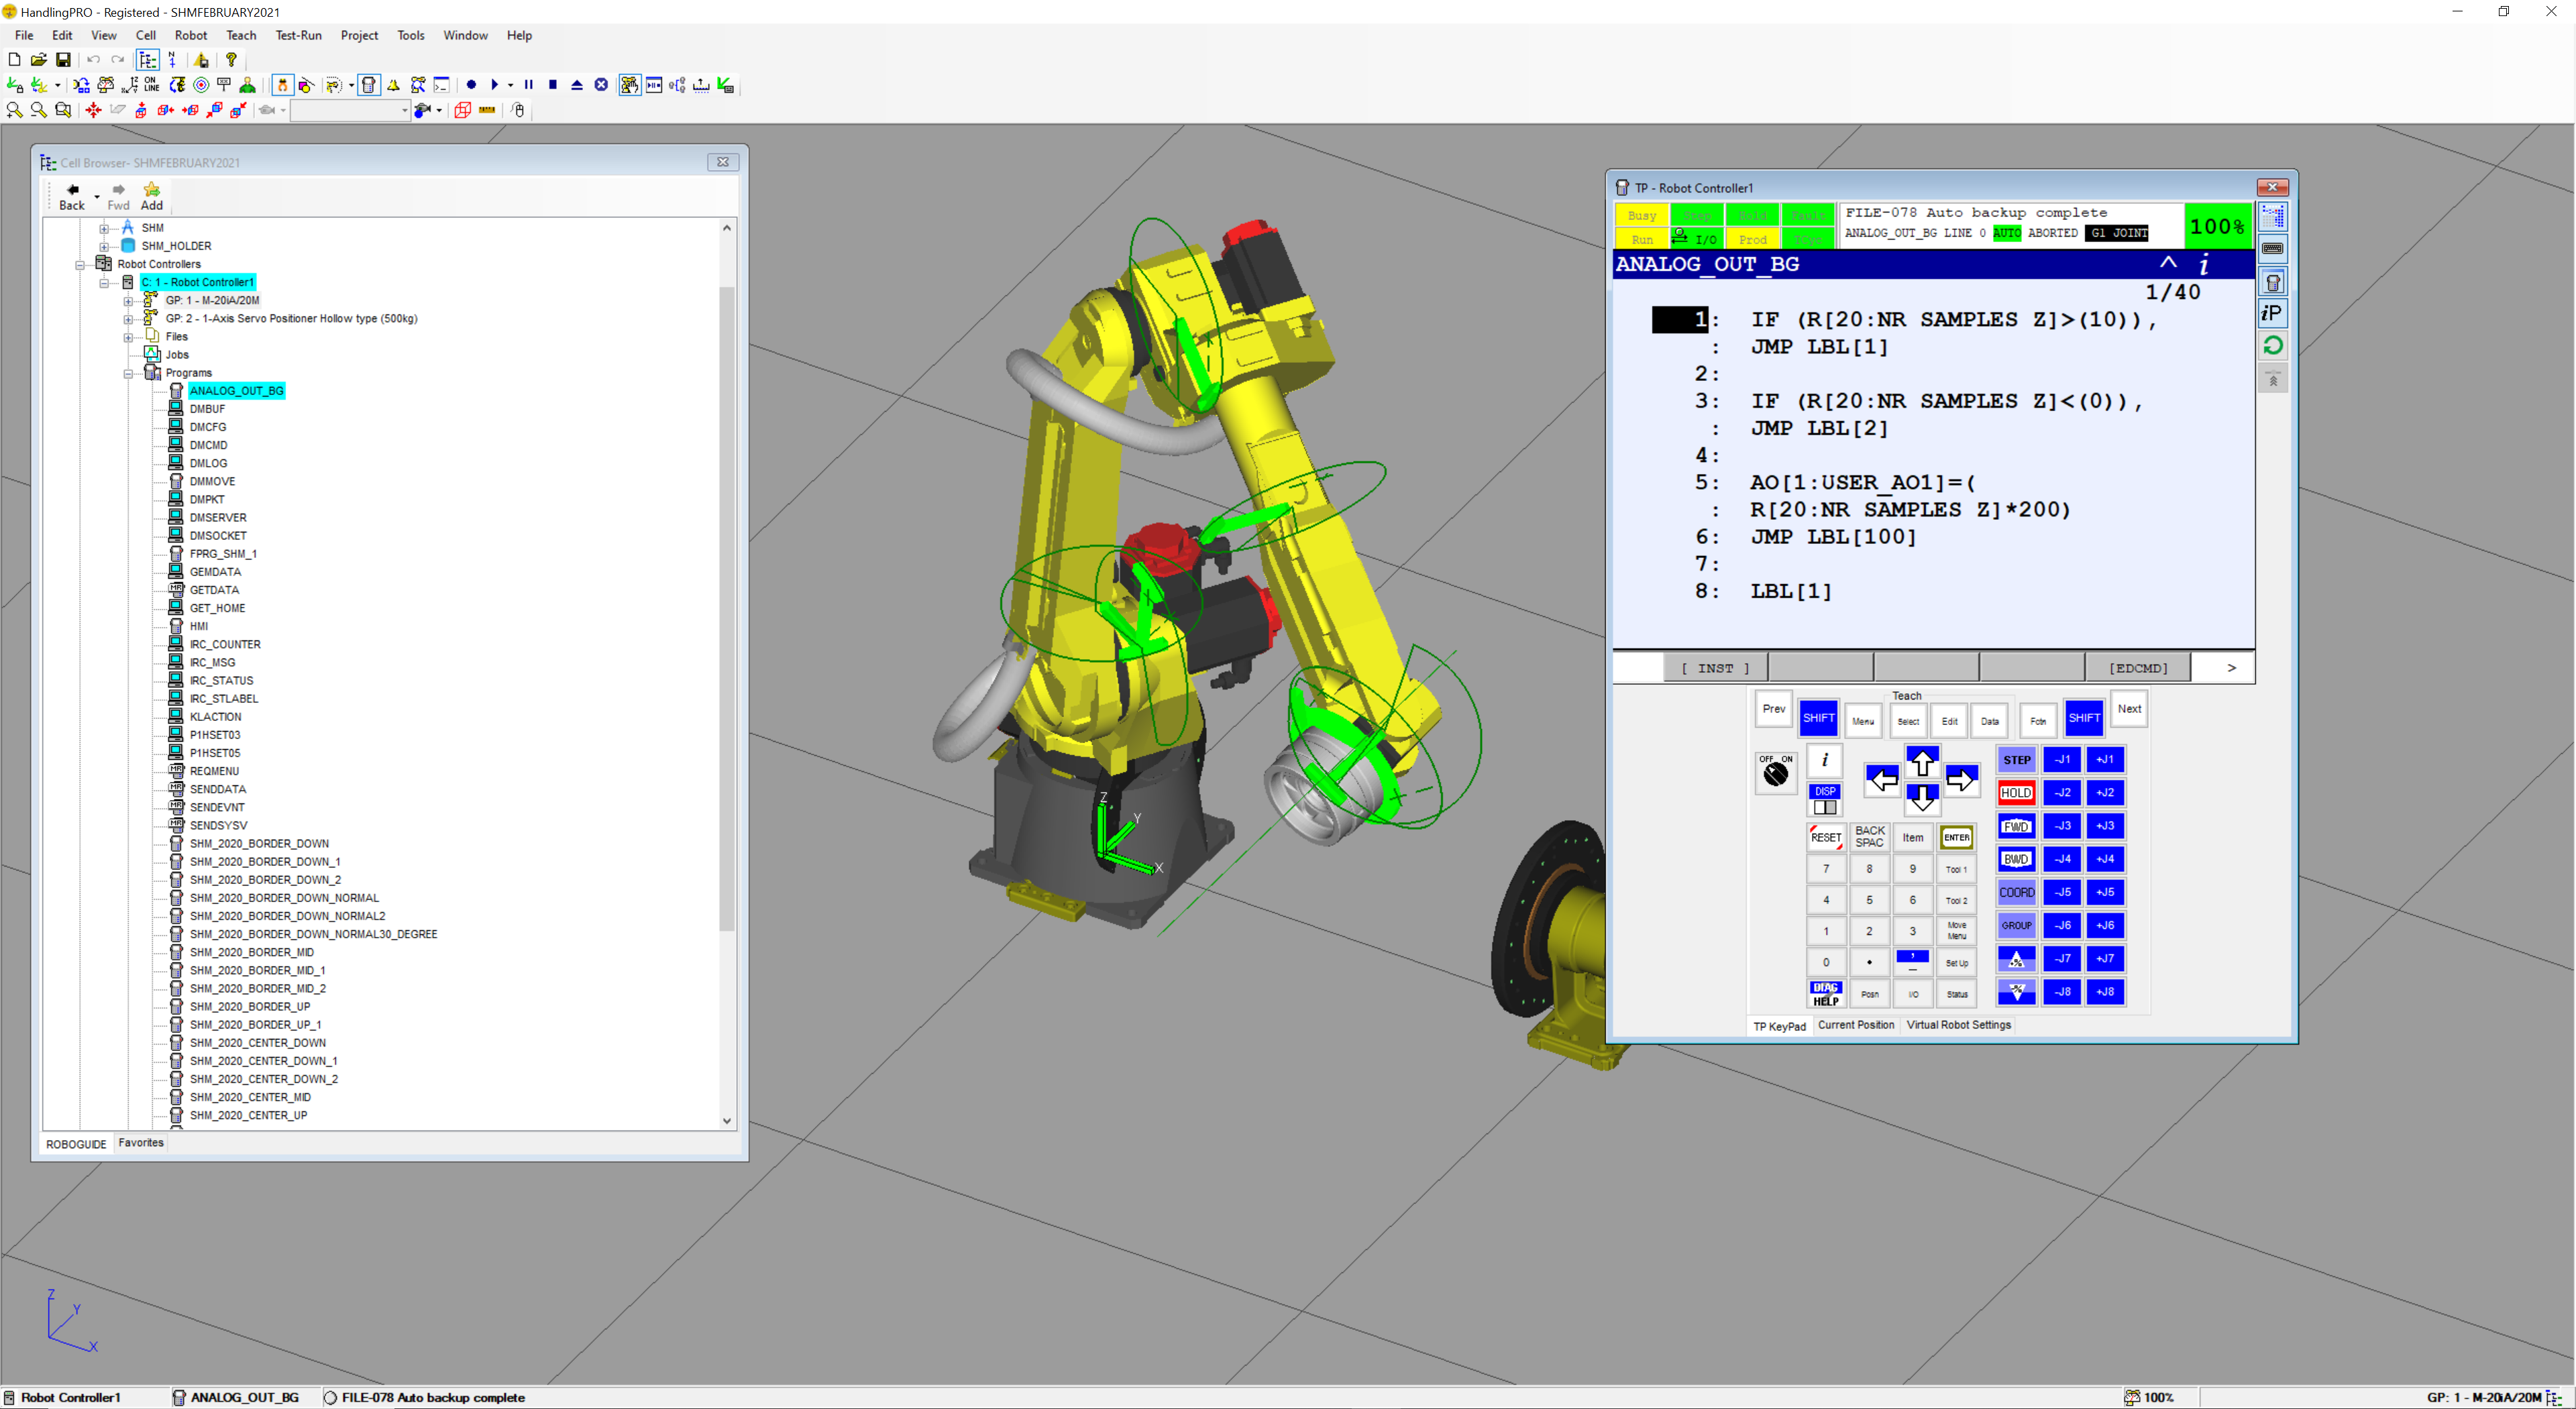
\includegraphics[width=0.9\linewidth]{img/roboguide.PNG}
    \caption{FANUC Roboguide workcell -- user interface example}
    \label{fig:roboguide}
\end{figure}

\subsection{FANUC robotic arm controller programming languages}

The FANUC company implements two programming languages for programming their robot controllers: teach pendant (TP) or KAREL. The TP language is mainly used for motion control of the robotic arm and the programs are usually edited via the pendant. TP programs are either binary files (\mintinline{shell-session}{.tp} file extension) or can be human--readable ASCII files (\mintinline{shell-session}{.ls} file extension). The KAREL language is a high--level language and does not support robotic arm movement instructions. KAREL is mainly used to implement program logic. KAREL programs can not be edited using a pendant.

\subsection{Compiling a FANUC TP program}

Only a TP program in binary format can be run on FANUC robotic arm controllers. Because RoboDK creates TP programs as human--readable ASCII files, the TP programs need to be converted to binary format before uploading them to the robot controller. Two options to convert \mintinline{shell-session}{.ls} programs to \mintinline{shell-session}{.tp} programs exist:

\begin{enumerate}
\item the ASCII Upload option must be loaded on the robot controller. After upload an \mintinline{shell-session}{.ls} file to the controller it is automatically converted to a \mintinline{shell-session}{.tp} file,
\item the program is compiled and uploaded either using the WinOLPC  tools via Roboguide or using the WinOLPC tools directly.

\end{enumerate}

\section{Robot machining projects in RoboDK}

The applications of robot machining in the industry are numerous. Some applications include:

\begin{itemize}

    \item milling,
    \item drilling,
    \item chamfering,
    \item deburring.

\end{itemize}

RoboDK offers three types of robot manufacturing projects:

\begin{itemize}

    \item robot machining projects,
    \item curve follow projects, 
    \item point follow projects. 

\end{itemize}

The process of setting up a curve follow project in RoboDK is described in the following sections. In laser shock peening, the laser (representing the tool) is static, and the robot holds the object. Therefore, a curve follow project with a constant tool orientation is set up in RoboDK.

\subsection{Setting up a curve follow project in RoboDK}

A curve follow project in RoboDK must at least consist of one robot, one tool, and one reference frame. The situation described is a so--called remote TCP situation, i.e., the Tool Center Point (TCP) is fixed in the station, and the robot holds the object. The TCP in our project is represented by the laser beam. 
The user has to execute the following steps to set up a basic curve follow project: 

\begin{enumerate}

\item create and import the robotic arm path to RoboDK using preferred CAD software,

\item mount the robot path as a tool in RoboDK,

\item import the robotic arm and create reference frame (optionally import CAD of manufactured part) into RoboDK station, 

\item create curve follow project: \mintinline{shell-session}{Utilities} $\rightarrow$ \mintinline{shell-session}{Curve follow project},

\item open the curve follow project settings. A window similar to the one displayed in Figure \ref{fig:curvefollow} will open, 

\item modify curve follow project settings:

    \begin{itemize}

        \item \mintinline{shell-session}{Robot}: the robotic arm holding the object,
        \item \mintinline{shell-session}{Reference}: the frame representing the remote TCP,
        \item \mintinline{shell-session}{Tool}: the robotic arm path.
        
    \end{itemize}
    
\item change \mintinline{shell-session}{Select algorithm} option to: \mintinline{shell-session}{Robot holds object & follows path},

\item update project. RoboDK automatically generates a preprocessed robot program for the actual station,

\item right--click the preprocessed program, select post processor and generate program. The \mintinline{shell-session}{.ls} program for the actual station will be opened in the default RoboDK text editor,

\item compile the program and export the program to the FANUC robot controller using Roboguide or WinOLPC tools.
    
\end{enumerate}

\begin{figure}[h]
    \centering
    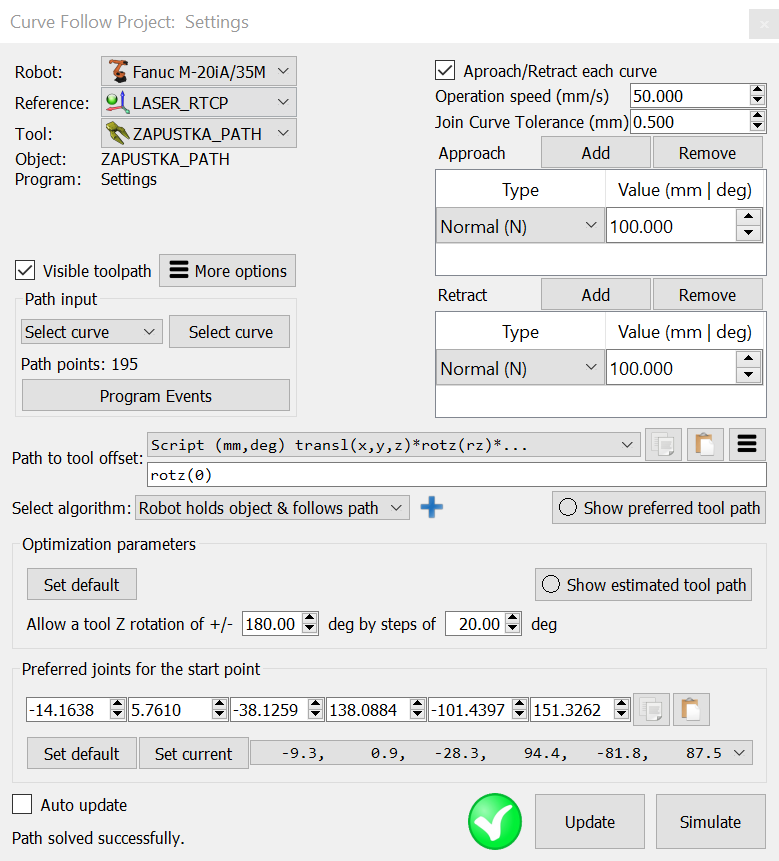
\includegraphics[width=0.9\linewidth]{img/curve_follow_settings.PNG}
    \caption{Curve follow project settings in RoboDK}
    \label{fig:curvefollow}
\end{figure}

\section{RoboDK API}

An application interface is a set of features an application provides to a user via a high--level programming language. The RoboDK API dramatically expands the possibilities of RoboDK. The RoboDK API is implemented in The RoboDK API is implemented in Python, C\#, C++, Visual Basic (.NET) and Matlab.  The Python API is the most extensive and is used in this thesis. The RoboDK API facilitates the execution of the following tasks:

\begin{itemize}
    
 \item Automating simulation -- macro scripts for repetitive tasks such as tool changing, pick and place applications.

 \item Offline programming -- using the RoboDK API methods to create programs for specific robotic arm controllers. The pre--processed \mintinline{shell-session}{.pyc} file created in RoboDK's GUI is executed directly by the post processor. The post processor defines the rules for vendor--specific robotic arm controller program generation. 

 \item Online programming -- using RoboDK API to move robots and retrieve their current position in real time. RoboDK connects to the robotic arm controller using robot drivers.

\end{itemize}

The elegance of this approach is that the same program written in a high--level programming language can be used for all three of the abovementioned tasks. 



\subsection{Python API for RoboDK}

Python is an interpreted high--level programming language. The Python API for RoboDK uses Python 3, although most features are compatible with Python 2 also. The RoboDK API for Python consists of the following modules:

\begin{itemize}
    \item \mintinline{text}{robolink} module -- this module represents the link between RoboDK and the high--level programming language,
    \item \mintinline{text}{item} module -- any item from the RoboDK item tree can be retrieved.  An item can be a robotic arm, a reference frame, a tool, an object, or a specific project,
    \item \mintinline{text}{robodk} module -- a module with a robotics toolbox for pose operations. All post processors depend on the \mintinline{text}{robodk} module \cite{robodkapi}.
\end{itemize}

The modules are located in the folder \mintinline{shell-session}{C:/RoboDK/Python/} in the Windows operating system. This folder is included in the \mintinline{shell-session}{PYTHONPATH} system variable. The Python API is accompanied with examples. These examples are located in the folders \mintinline{shell-session}{C:/RoboDK/Library/Scripts}  and \mintinline{shell-session}{C:/RoboDK/Library/Macros}  in the Windows operating system.

\section{RoboDK post processors}

A post processor specifies how robot programs must be generated for a specific robot controller and are used when robotic arm controllers are generated offline. Post processors serve as tools to convert the simulation to vendor--specific robot programs. All RoboDK post processors are placed in the \mintinline{shell-session}{C:/RoboDK/Posts} folder in the Windows operating system. All post processors rely on the \mintinline{shell-session}{robodk} module. The \mintinline{shell-session}{robodk} module is a robotics toolbox for Python, based on \href{http://petercorke.com/Robotics_Toolbox.html}{Peter Corke’s Robotics Toolbox}. 

\subsection{RoboDK preprocessed file}

After creating a program in the curve follow project, but before generating it using a post processor, the program is saved as a preprocessed/universal Python program and saved in a local temporary folder. The preprocessed program is linked to the right post processor (selected by the user in RoboDK). The post processor defines a \mintinline{python}{RobotPost} class that generates the desired code. In the Windows operating system, the preprocessed Python files are saved in the user's temporary folder (e.g.: \mintinline{shell-session}{C:/Users/username/AppData/Local/Temp}) folder. These programs can also be used for debugging new post processors. An example code of a preprocessed file is shown in Listing \ref{code:preprocessed_python}:

%% this is an example of a minted code with caption and wrapped lines
\begin{code}
\label{code:preprocessed_python}
\begin{minted}[frame=lines, linenos,tabsize=2,breaklines]{python}
import sys
import os
sys.path.append(os.path.abspath(r"""C:/RoboDK/Posts/""")) # temporarily add path to POSTS folder

from FANUC_R30iA_decompyle3 import *

def p(x,y,z,r,p,w):
  a = r*math.pi/180.0
  b = p*math.pi/180.0
  c = w*math.pi/180.0
  ca = math.cos(a)
  sa = math.sin(a)
  cb = math.cos(b)
  sb = math.sin(b)
  cc = math.cos(c)
  sc = math.sin(c)
  return Mat([[cb*ca,ca*sc*sb--cc*sa,sc*sa+cc*ca*sb,x], [cb*sa,cc*ca+sc*sb*sa,cc*sb*sa--ca*sc,y], [--sb,cb*sc,cc*cb,z], [0.0,0.0,0.0,1.0]])

print('Total instructions: 140')
r = RobotPost(r"""FANUC_R30iA_decompyle3""",r"""Fanuc M--20iA/35M""",6, axes_type=['R','R','R','R','R','R'], ip_com=r"""127.0.0.1""", api_port=20500, prog_ptr=2172227036784, robot_ptr=2172252511552)

r.ProgStart(r"""Settings""")
r.RunMessage(r"""Program generated by RoboDK v5.2.2 for Fanuc M--20iA/35M on 02/07/2021 17:12:29""",True)
r.RunMessage(r"""Using nominal kinematics.""",True)
r.setZoneData(1.000)
r.setSpeed(1000.000)
r.setFrame(p(1000.3,--445,552.3,0,10.19,--90),--1,r"""LASER_RTCP""")
r.setTool(p(0,0,0,0,0,0),--1,r"""ZAPUSTKA_PATH""")
r.RunMessage(r"""Show ZAPUSTKA_PATH""",True)
r.MoveJ(None,[--9.2878,0.949114,--28.3094,94.4347,--81.8311,87.4811],None)
r.MoveL(p(--14.8303,41.4662,85,105.917,0,180), [--14.8823,2.45519,--28.2667,97.1731,--76.9261,87.0176], [0,0,0])
r.setSpeed(10.000)
r.MoveL(p(0.866853,42.1343,85,94.455,0,180), [--14.6627,3.59506,--28.447,97.1044,--77.1403,75.3963], [0,0,0])
r.MoveL(p(11.9961,40.7679,85,85.5416,0,--180), [--14.5062,4.37964,--28.4381,97.0241,--77.2757,66.5094], [0,0,0])
r.MoveL(p(16.6541,40.7679,85,85.5416,0,180), [--14.4431,4.71382,--28.4699,96.9996,--77.3347,66.484], [0,0,0])

...
...
...

r.MoveL(p(--16.8929,40.7854,85,108.509,0,180), [--14.9101,2.29849,--28.2014,97.1719,--76.8936,449.673], [0,0,0])
r.setSpeed(1000.000)
r.MoveL(p(--16.1785,41.074,185,107.509,0,180), [--9.29955,0.844572,--28.2678,94.4344,--81.8176,449.114], [0,0,0])
r.ProgFinish(r"""Settings""")
r.ProgSave(r"""C:/Users/marek.boehm/Documents/RoboDK/""", r"""Settings""", False, r"""C:/RoboDK/Other/VSCodium/VSCodium.exe""")

\end{minted}
\captionof{listing}{Snippet of preprocessed program to be executed by post processor}
\end{code}

Let us dive into the source code of this preprocessed file and explain the functionality of some of its methods. The \mintinline{python}{p(x,y,z,r,p,w)} function converts the XYZRPW representation to a Pose ($ 4 \times 4 $ matrix). The \mintinline{python}{RobotPost} class initializes the robot post processor object. The parameters of the \mintinline{python}{RobotPost} class are:

\begin{code}
\begin{minted}[frame=lines,tabsize=2,breaklines]{python}

class samplepost.RobotPost(robotpost=None, robotname=None, robot_axes=6, **kwargs)

\end{minted}
\end{code}

Parameters of \mintinline{text}{RobotPost} class:

\begin{itemize}

\item \mintinline{python}{robotpost (string)} -- name of the post processor linked to the preprocessed file,

%% do not highlight anything - then use text
\item \mintinline{text}{robotname(string)} -- the name of the robotic arm,

\item \mintinline{text}{robotaxes(string list)} -- type and quantity of robotic arm axes,

\item \mintinline{text}{**kwargs} -- pass additional arguments to function.

\end{itemize}

All subsequent functions are called upon the \mintinline{python}{RobotPost} object. The most important function is the \mintinline{python}{MoveL} function:

\begin{code}
\begin{minted}[frame=lines,tabsize=2,breaklines]{python}

MoveL(pose, joints, conf_RLF=None)

\end{minted}
\end{code}

Parameters \mintinline{text}{MoveL} method:

\begin{itemize}

\item \mintinline{text}{pose (robodk.Mat())} -- pose target of the tool with respect to the reference frame, pose can be \mintinline{python}{None} if the target is defined as a joint target,

%% do not highlight anything - then use text
\item \mintinline{text}{joints (float list)} -- robot joints as a list,

\item \mintinline{text}{robotaxes(array)} -- type and quantity of robotic arm axes,

\item \mintinline{text}{conf_RLF (int list)} -- pass additional arguments to function. 

\end{itemize}

Another important method in the preprocessed file is the \mintinline{python}{ProgSave} method, which saves the program after all instructions have been executed:

\begin{code}
\begin{minted}[frame=lines,tabsize=2,breaklines]{python}

ProgSave(folder, progname, ask_user=False, show_result=False)

\end{minted}
\end{code}

Parameters of \mintinline{text}{ProgSave} method:

\begin{itemize}

\item \mintinline{text}{pose (robodk.Mat())} -- pose target of the tool with respect to the reference frame, pose can be \mintinline{python}{None} if the target is defined as a joint target,

%% do not highlight anything - then use text
\item \mintinline{text}{folder (str)} -- folder hint to save the program,

\item \mintinline{text}{progname (str)} -- program name as a hint to save the program,

\item \mintinline{text}{ask_user (bool, str)} -- true if the default settings in RoboDK are set to promt the user to select the folder, 

\item \mintinline{text}{show_result (bool, str)} -- false if the default settings in RoboDK are set to not show the program once it has been saved. Otherwise, a string is provided with the path of the preferred text editor.

\end{itemize}

 Every post processor should implement a set of basic methods to generate programs for robotic arm controllers correctly. These basic  methods used in the preprocessed file can be found in the \href{https://robodk.com/doc/en/PythonAPI/postprocessor.html#post-processor-methods}{online documentation}.


\subsection{Selecting a post processor}

Each robotic arm has a post processor assigned to it by default. The following steps have to be taken to change the post processor of a robotic arm:


\begin{itemize}
    \item opening the robot panel,
    \item selecting \mintinline{shell-session}{Parameters},
    \item selecting post processor from drop--list.
\end{itemize}

\subsection{Post processor example and example output}

????Here put a link to you github repo, or a snippet????


\subsection{FANUC R--30iA post processor}

The FANUC R--30iB post processor is located in the \mintinline{shell-session}{C:/RoboDK/Posts/vXX folder}. \mintinline{shell-session}{XX} is a two--digit number and denotes the post processor version. The FANUC R--30iA post processor comes in the form of a \mintinline{shell-session}{.pyc} file (compiled bytecode) and needs to be decompiled to a \mintinline{shell-session}{.py} file with the help of a decompiler. The decompyler used in this thesis is   \href{https://github.com/rocky/python--decompile3}{decompyle3}.

\section{Modifying the FANUC R--30iB post processor methods} 

The user can create a new post processor from scratch or modify an existing post processor. A post processor for a specific robotic arm controller is a single \mintinline{shell-session}{.py} file. All post processors are placed in the \mintinline{shell-session}{C:/RoboDK/Posts} folder. A new post processor is added to RoboDK by creating a \mintinline{shell-session}{.py} file or renaming an existing \mintinline{shell-session}{.py} file in this folder. By deleting a \mintinline{shell-session}{.py} file in this folder, the post processor is deleted from the list of post processors in RoboDK. 

The experimental setup of the LSP station at the HiLASE centre links the robotic arm controller to the laser source. The objective of the post processor modification can be expressed as:

The laser source is operating at 1 Hz repetition rate. The post processor for the  R--30iB controller will be modified in such a way that when the robotic arm with the sample is in a position, where the LSP process (individual laser impact area) should be placed, the robotic arm controller sends a command to the laser source to fire exactly one laser pulse onto the desired area and then move on to the next position. This is accomplished by controlling the digital inputs (DIs) and digital outputs (DOs) of the robotic arm controller. 

The modification involves the MoveL method. The original MoveL method generates the following code:

L P[X] Ymm/sec CNT100

where:
L
P[X]
Ymm/sec
CNT100

The modified MoveL method should output the following robotic arm controller code to meet the requirements on the post processor:

  :WAIT DI[1:SYNCHRONIZATION_IN]=OFF   ;
  :WAIT DI[1:SYNCHRONIZATION_IN]=ON    ;
  :L P[6] 4mm/sec CNT100 RTCP TB  0.00sec,DO[5]=PULSE,1.0sec;
  :WAIT  DO[5:LASER ON] = OFF ;
  :WAIT  1.00(sec) ;

where:

Listing contains the original MoveL method of the FANUC R--30iB post processor. 

HERE WRITE ABOUT THE MODIFIED METHOD.


